% $Id: Field_usage.tex,v 1.3 2003/11/14 20:53:10 jwolfe Exp $

%\subsection{Design}

% <Describe strategy for overall class design.>


The Field class aggregates two internal subclasses: a GlobalField class
and a LocalField class.  This separation allows the code to clearly
differentiate between functions which operate internal to a single DE
on a local decomposition of data, 
and those which must be aware of the
global state of the Field.  
 
There is a correspondence between the Global Distributed Grid class,
and the Local Distributed Grid class, and Fields.  Each DE contains
the corresponding local decompositions for Distributed Grids and Fields.

The Field class maintains the relationship of
how data maps onto the grid (e.g. one item per cell located at
the cell center, one item per cell located at the NW corner, 
one item per cell vertex, etc).  This means that different Fields
which are on the same underlying Grid but have different
mappings (staggerings) can share the same Grid object without
needing to copy or replicate it multiple times.  Regridding
operations can operate first on the shared Grid, and then
use the staggering information from the Field to compute the
corresponding transformation of the data.

Some methods which have a Field interface will actually be
implemented at the underlying Grid or Array level; they
will be inherited by the Field class.  This allows the user
API (Application Programming Interface) to present functions at
the level which is most consistent to the application without
restricting where inside the ESMF the actual implementation
is done.


% cecelia - this is the new section on the data interfaces to the
% communications routines.  move it where you want.   nsc 31jul03

\subsection{Distributed Data Methods}

There are ten methods which involve movement of data between DEs.
The first three are higher level functions which are intended to
map closely to needs of applications programs.  They are:

\subsubsection{Halo}
% $Id: ArrayHalo_desc.tex,v 1.3 2004/06/03 22:33:15 cdeluca Exp $

\label{sec:halo}
Halo operations update ghost cell or halo regions at the boundaries
of a local data decomposition.  Halo regions are to be considered
read-only by the local process; their data values can be used to
compute the new values for cells which are local to this process,
but they cannot be updated except by a halo operation.  Haloing is
supported at the Array and Field level.  

\subsection{Halo Domains}

Array objects can have an optional {\bf halo width} which defines
what part of the Array is the {\bf exclusive domain}, the {\bf computational
domain}, and the {\bf total domain}.  With no halo region, all these are
the same and equal to the total size of the Array.  The domains are
defined as follows.

\begin{itemize}

\item {\bf Exclusive}  The exclusive domain is the subset of the
Array which is never read by any other DE.  

\item {\bf Computational}  The computational domain
is the subset of the Array which is read and written by the current DE.

\item {\bf Total}  The total domain includes the region where data is 
updated from another DE during a halo operation and read but not 
updated by the current DE.  

\end{itemize}

Figure \ref{fig:halo} illustrates these concepts.

Halo domain information must be stored at the Array level to
support operations such as the gather, which collects
decomposed parts of a logically contiguous object onto a single DE.
Only the computational domain is copied since the halo regions are
duplicated data.  The exclusive domain is guaranteed to never be
the source of data for a halo operation, so no synchronization
of updates to those data items needs to be done.  The total
domain is the actual memory size allocated for the Array,
and is used when computing offsets for subdomains within the Array.

\begin{center}
\begin{figure}
\caption{Diagram showing how ESMF exclusive, computational,
and total domains are defined.  }
\label{fig:halo}
\scalebox{1.0}{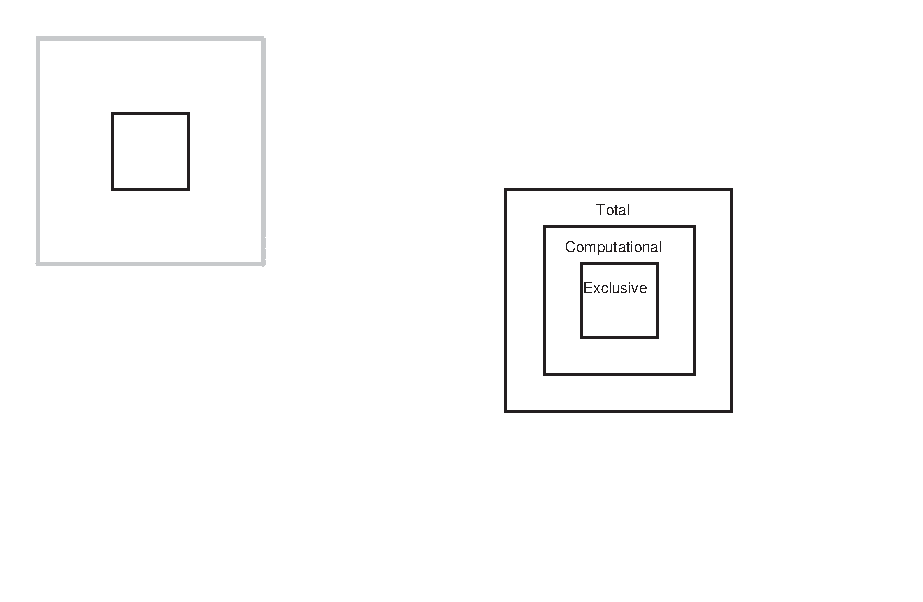
\includegraphics{Field_halo.eps}}
\end{figure}
\end{center}




\subsubsection{Regrid}
% $Id: Regrid_usage.tex,v 1.15 2006/02/01 19:10:46 cdeluca Exp $


Regrid is designed to be called with Field or Bundle
arguments in order to utilize information embedded in
these objects.  For example, Regrid requires knowledge
of underlying grid information (both PhysGrid and DistGrid)
and of the relative location (staggering) of Fields on
the Grid.  In addition, Regrid uses any mask information
that may be associated with a Field.  However, ESMF also
provides an Array interface for users who have gathered all
necessary information.

Regrid is separated into RegridStore functions, a Regrid
function, and a RegridRelease function. The Store functions
compute interpolation weights and initialize communication
requirements for performing a regridding of a Field
from one Grid to another, returning an object called an
{\tt ESMF\_RouteHandle}.  The Regrid function uses
the created RouteHandle object to perform the actual regridding
of Fields or Bundles.  The Release function deletes the
RouteHandle object and frees all memory associated with a Regrid.
The reason for the separation is that in many cases, the
initial creation is expensive and re-used often throughout
an application.  The Regrid and RegridRelease functions are
also common to all the Regrid methods.

Because many methods are supported for regridding,
the main Store function branches to a specific
creation function based on the regrid method requested
(e.g. bilinear, conservative, spectral).  Each of
these regrid methods are in a separate module to
prevent the main Regrid module from becoming too
large.  The user is unaware of this hierarchy as the
top-level module provides a unified API.

In general, Regrid interfaces are relatively simple and require little
information directly from users.  Besides prescribing the actual Regrid method,
they offer users few options, as shown in the example in
Section~\ref{sec:RegridExamples}.  However, the simplicity of the interfaces
belies the complicated nature of the underlying code.  ESMF endeavors to hide as
much of this complication from its users as possible.  However, Regrid does have
current limitations that require user awareness to successfully use its
routines.  These issues are discussed below.

\subsubsection{Regrid and Grid Overlap}

Regrid assumes both the source and destination Grids share the same coordinate
system and units.  Although 3D regridding is not yet available, this rule is
also expected to be valid for vertical grids as well.  At this point, the ESMF
definition of a common coordinate system includes the extents used to define
a domain.  For example, Regrid routines do not understand that latitudes from
-180 to +180 degrees and latitudes from 0 to 360 degrees are describing the
same domain with a different range.  Currently, users are responsible for any
necessary conversion or translation.  

There are five possible physical overlap situations between the source and
destination Grids, illustrated in Figure~\ref{fig:RegridGridOverlap}.

\begin{center}
\begin{figure}
\scalebox{0.9}{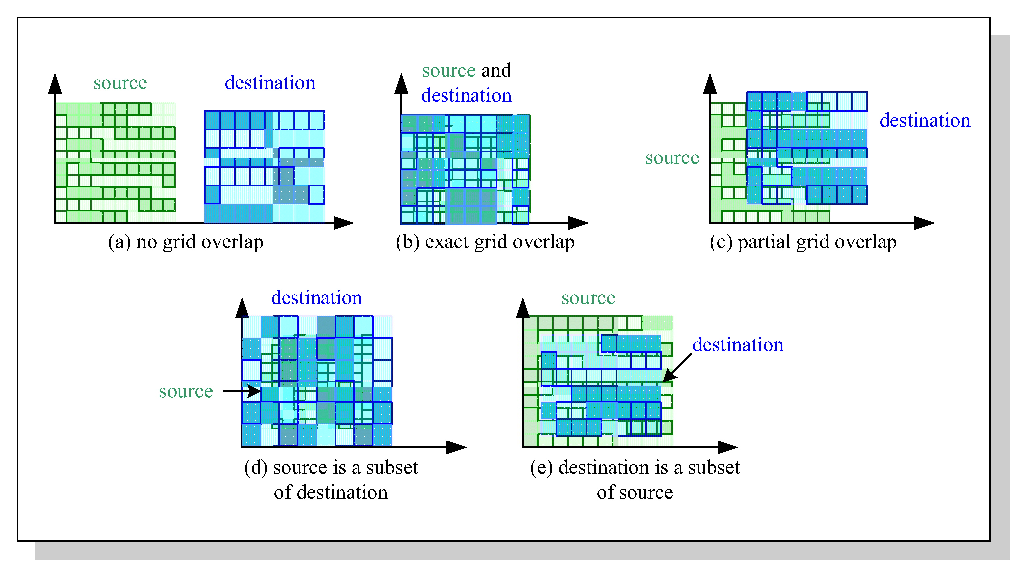
\includegraphics{RegridGridOverlap}}
\caption{Possible Relationships between Grids in Physical (Coordinate) Space. }
\label{fig:RegridGridOverlap}
\end{figure}
\end{center}

Regrid can provide complete interpolation weights for the destination Field
only for those situations where there is source data covering the entire physical
domain of the destination Grid (cases (b) and (e) above).  In all the other
cases, there are parts of the destination Grid for which there is no source. 
When source data is not available, Regrid routines will not extrapolate data
values and the destination Field may contain data points that have not been
calculated or filled.  Currently, regrid routines initialize the destination
Field to a value of zero prior to regridding, so unfilled destination data points
will have that value.  In the future, regrid routines will have an optional
argument allowing users to specify a fill value besides zero.  


\subsubsection{Regrid and Data Location}

There is no restriction in Regrid that the source and destination Fields
define their data in the same relative location (RelLoc).  However, regridding
between Fields with different RelLocs can have unintended consequences if the
related Grids cover exactly the same physical domain.  The RelLocs represent
different subGrids, which can shift the represented physical domain by plus or
minus one-half of a cell width.  This is illustrated below in
Figure~\ref{fig:RegridRelLocEffect}, which shows the physical areas described by
two sample RelLocs and the effect on the overlap of the global Grids.  In this
situation, there may be some unfilled or less accurate Field data at some of the
Grid boundaries.

\begin{center}
\begin{figure}
\scalebox{0.9}{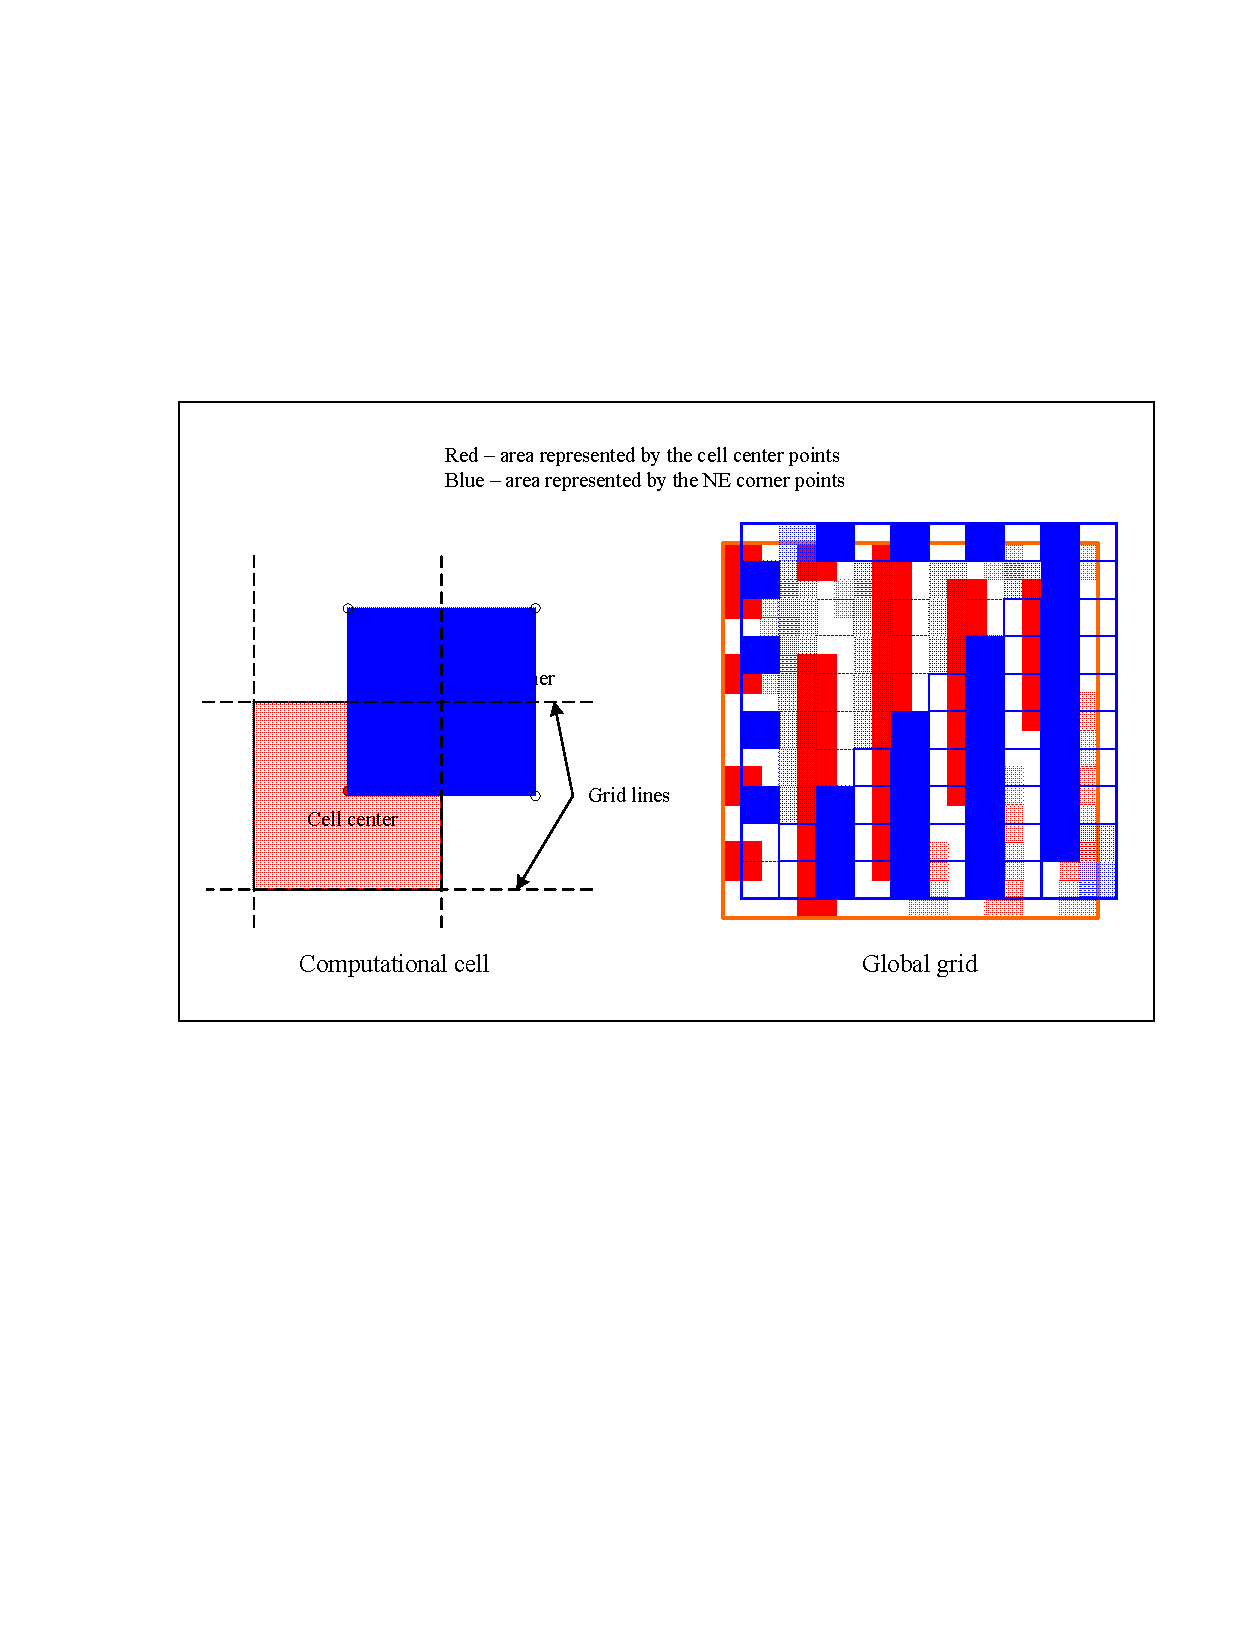
\includegraphics{RegridRelLocEffect}}
\caption{Illustration of Grid areas represented by differing RelLocs. }
\label{fig:RegridRelLocEffect}
\end{figure}
\end{center}

\subsubsection{Regrid and Grid Refinement}

Different refinement or cell sizes (also called resolution) between the source
and destination Grids may have a similar effect on regridding as does different
data locations. This can be true even if the source and destination Fields have
the same RelLoc, as illustrated in Figure~\ref{fig:RegridRefinementEffect}.  In
this diagram, the areas of the two grids represented by the corresponding Fields do not overlap
exactly despite sharing identical physical extents and relative data locations.
Again, this situation may cause some inaccuracy in the regridded Field data at
the Grid boundaries.

\begin{center}
\begin{figure}
\scalebox{0.9}{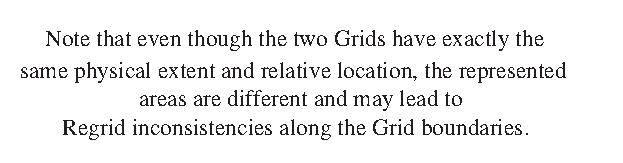
\includegraphics{RegridRefinementEffect}}
\caption{Illustration of areas represented by the same RelLoc on Grids with
          different refinement. }
\label{fig:RegridRefinementEffect}
\end{figure}
\end{center}


\subsubsection{Regrid and Periodicity}

Some of the Regrid issues raised in the previous sections concerning the effect
of data locations and Grid refinement are negated by the integration of
periodic boundary conditions into Regrid routines.  As illustrated in
Figure~\ref{fig:RegridPeriodicity}, areas represented by Field data that
would otherwise extend beyond the nominal Grid boundaries are mapped or "wrapped"
back onto the Grid at the corresponding periodic boundary.  This effectively 
ensures complete overlap for Grids that share identical physical extents.

\begin{center}
\begin{figure}
\scalebox{0.9}{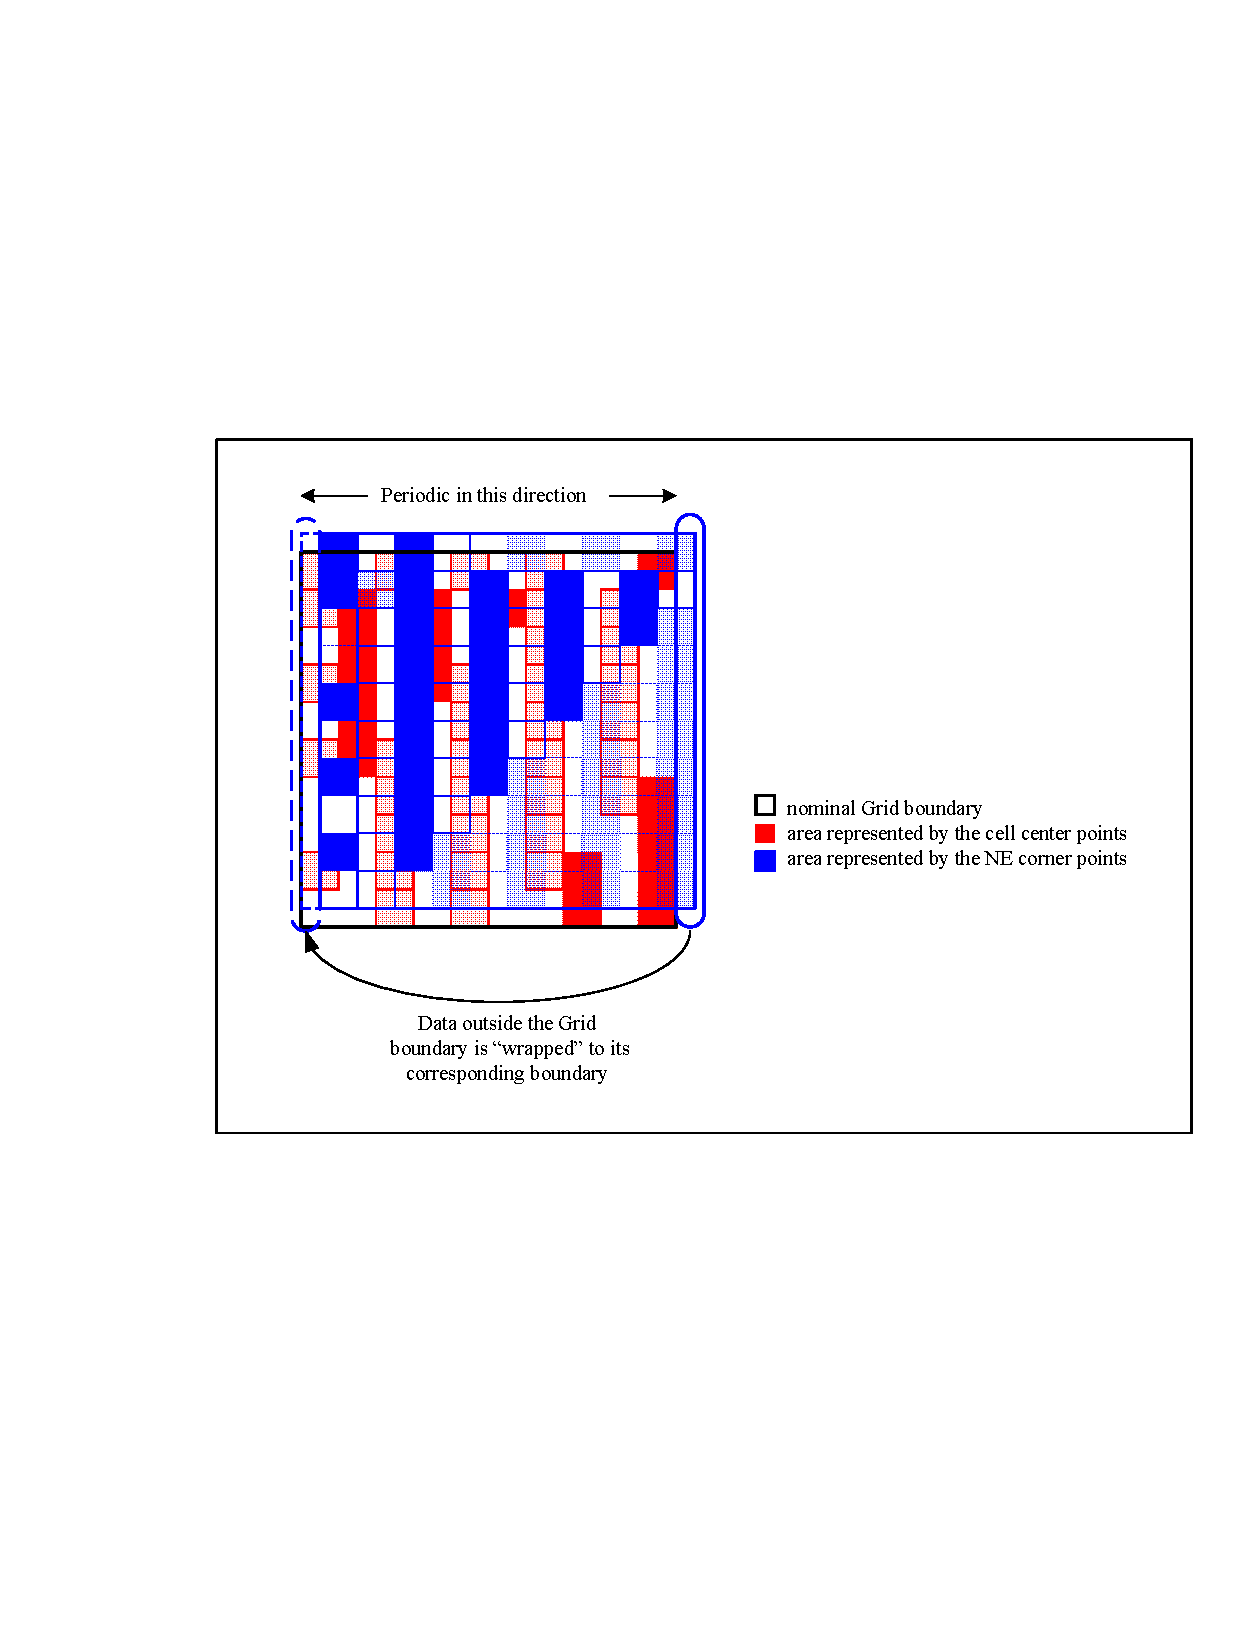
\includegraphics{RegridPeriodicity}}
\caption{Illustration of Regrid Overlap issues solved by the implementation
          of periodic boundary conditions. }
\label{fig:RegridPeriodicity}
\end{figure}
\end{center}

Unfortunately, the Regrid routines in ESMF do not currently include periodic
boundary effects, so users must be aware of possible problems.


\subsubsection{Regrid Examples: Precomputing and Executing a Regrid}
\label{sec:RegridExamples}

The following code fragments show an example of the steps involved in
computing and applying a Regrid.




\subsubsection{Redist}
% $Id: ArrayRedist_desc.tex,v 1.7 2005/12/21 23:23:23 jwolfe Exp $


As the name implies, Redistribution operations move data from one distribution,
or decomposition, to another.  The distribution of the data may differ in several 
ways:
 \begin{description}

  \item The data could be decomposed across multiple DEs differently.  In this
        case, the source data might be decomposed by a 3 by 2 DELayout and be
        redistributed onto a 1 by 6 DELayout.

  \item The data could have different index orderings.  For example, the data
        might be reordered from IJK to KIJ, where the source data is
        dimensioned srcData(ni,nj,nk) and is redistributed to dstData(nk,ni,nj).

  \item Different indices of the data could be decomposed.  Source data
        decomposed only in the first index could be redistributed to being
        only in the second or third index.  For example, if both the source
        and destination data are decomposed by a 4 by 1 DELayout but the source
        applies the decomposition to the first index and the destination
        applies it to the second, then the source data will be locally
        dimensioned srcData(ni/4,nj,nk) and redistributed to dstData(ni,nj/4,nk).

 \end{description}

In all of these situations, the source and destination data structures are
required to have identical global sizes but not DE-local sizes.  Although
illustrations of Redistribution may look very similar to Regridding (please
see Figure \ref{fig:Redist}),

\begin{center}
\begin{figure}
\label{fig:Redist}
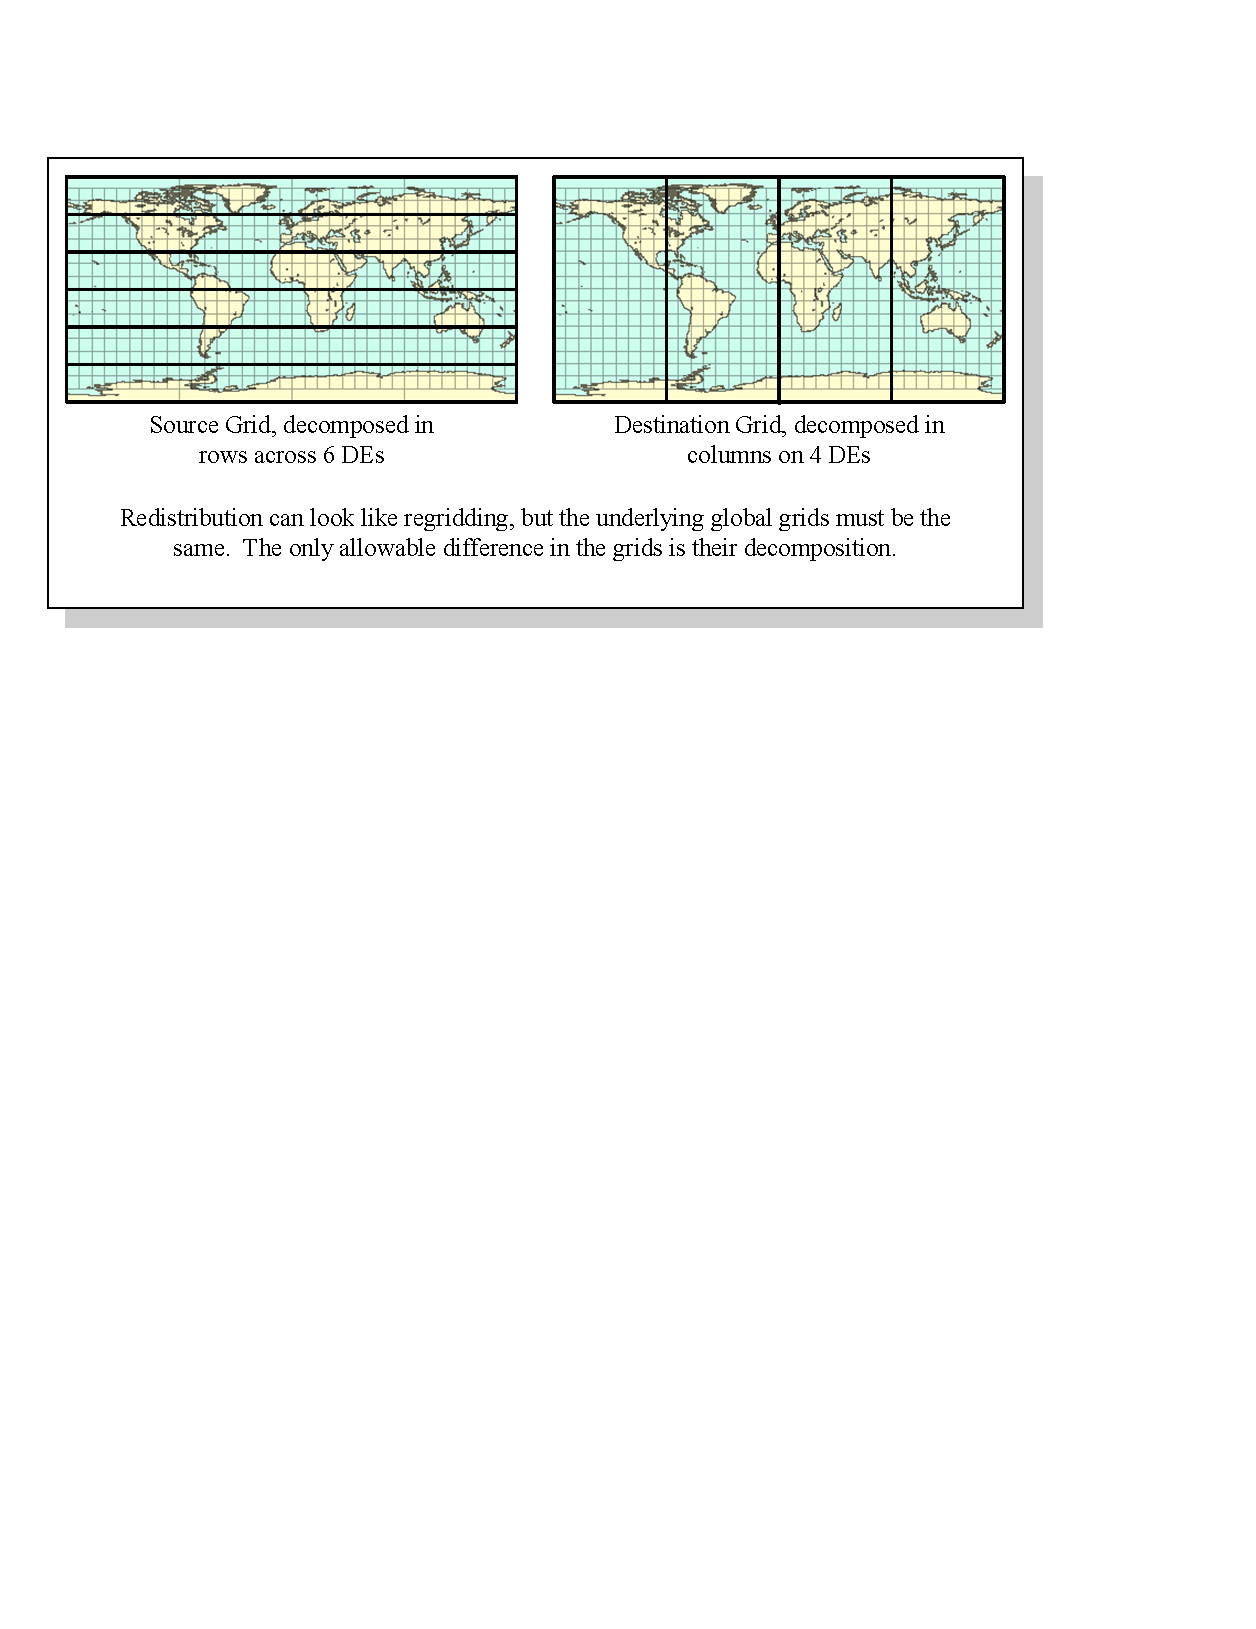
\includegraphics{Redist}
\caption{Illustration of redistribution of data. }
\end{figure}
\end{center}

Redistribution methods involve only data movement; no interpolation, data
binning, or averaging is performed.  For data associated with physical locations
on a Grid, this means the source and destination Grids must have identical
global coordinates.  Like Haloing and other high level communication routines,
Redistribution is supported at the Array, Field, and Bundle levels. 



\subsubsection{Lower Level Functions}
The last seven correspond closely to the lower level
MPI communications primitives.  They are:
\begin{description}
\item[Gather]
Reassembling data which is decomposed over a set of DEs into a single
block of data on one DE.
\item[AllGather]
Reassembling data which is decomposed over a set of DEs into multiple
copies of a single block of data, one copy per original DE.
\item[Scatter]
Spreading an undecomposed block of data on one DE over a set of DEs,
decomposing that single block into smaller subsets of data, one
data decomposition per DE.
\item[AlltoAll]
Spreading an undecomposed block of data from multiple DEs onto
each of the other DEs in the set, resulting in a set of multiple decomposed 
data blocks per DE, one from each of the original source DEs.
\item[Broadcast]
Spreading an undecomposed block of data from one DE onto all other
DEs, where the resulting data is still undecomposed and simply
copied to all other DEs.
\item[Reduction]
Computing a single data value, e.g. the data maximum, minimum, sum, etc
from a group of decomposed data blocks across a set of DEs, where the
result is delivered to a single DE.
\item[AllReduce]
Computing a single data value, e.g. the data maximum, minimum, sum, etc
from a group of decomposed data blocks across a set of DEs, where the
result is delivered to all DEs in the set.
\end{description}

Each of these methods can be called on Bundles, with and without packed
data, on Fields, and on Arrays.

